%%%%%%%%%%%%%%%%%%%%%%%%%%%%%%%%%%%%%%%%%
% Beamer Presentation
% LaTeX Template
% Version 1.0 (10/11/12)
%
% This template has been downloaded from:
% http://www.LaTeXTemplates.com
%
% License:
% CC BY-NC-SA 3.0 (http://creativecommons.org/licenses/by-nc-sa/3.0/)
%
%%%%%%%%%%%%%%%%%%%%%%%%%%%%%%%%%%%%%%%%%

%----------------------------------------------------------------------------------------
%	PACKAGES AND THEMES
%---------------------------------------------------------------------------------------

\documentclass{beamer}
\usepackage[spanish]{babel}
\usepackage{algpseudocode}
\usepackage[utf8]{inputenc}
\mode<presentation> {
	
	
	\usetheme{PaloAlto}
	
}

\usepackage{graphicx} % Allows including images


%----------------------------------------------------------------------------------------
%	TITLE PAGE
%----------------------------------------------------------------------------------------

\title[Práctica 4]{TSP} % The short title appears at the bottom of every slide, the full title is only on the title page

\author{Algorítmica} % Your name
\institute[UGR] % Your institution as it will appear on the bottom of every slide, may be shorthand to save space
{
	Universidad de Granada \\ % Your institution for the title page
	\medskip
	
}
\date{\today} % Date, can be changed to a custom date

\begin{document}
	
	\begin{frame}
		\titlepage % Print the title page as the first slide
	\end{frame}
	
	\begin{frame}
		\frametitle{Índice} % Table of contents slide, comment this block out to remove it
		\tableofcontents % Throughout your presentation, if you choose to use \section{} and \subsection{} commands, these will automatically be printed on this slide as an overview of your presentation
	\end{frame}
	
	%----------------------------------------------------------------------------------------
	%	PRESENTATION SLIDES
	%----------------------------------------------------------------------------------------
	
	\section{Introducción }
	\begin{frame}
		\frametitle{Introducción}
		\begin{itemize}
			\item El objetivo de esta práctica es resolver el problema del TSP utilizando para ello un enfoque Branch and Bound y, alternativamente, otro con Backtracking y comparar ambos.
		\end{itemize}
	\end{frame}
	
	


\begin{frame}
		\section{Representación de la solución} 
				\frametitle{Representación de la solución}
		
		Vector de tamaño N en el que el índice del vector nos indica el orden en el que las ciudades deben de ser visitadas y el contenido de cada posición hace referencia al índice de la ciudad
	\end{frame}
	%------------------------------------------------
\section{Diseño del algoritmo: Branch and Bound} 
\begin{frame}
	\frametitle{Diseño del algoritmo}
	


Usaremos una cola con prioridad que será donde se introduzcan los nodos.
En la cola se seleccionará el nodo con mayor prioridad, y de dicho nodo se consultará el valor de su cota local, que en caso de ser mejor a la global  y ser nodo hoja, se actualizará la solucion, en caso sólo de ser mejor que la global, se añadiran los hijos del nodo a la cola. En caso de ser peor, se devuelve la solucion actual.


	
\end{frame}	
	\section{Pseudocódigo}
	
	\begin{frame}
		\frametitle{Pseudocódigo}
		\footnotesize{	
			\begin{algorithmic}				
				\Require Matriz\_costes, Vector\_ciudades[N] Vector\_distancias\_minimas; 
				\State \textbf{Branch\&Bound( Matriz\_costes, Vector\_ciudades Vector\_distancias\_minimas):}
				\State priority\_queue cola;
				\State solucion\_final;
				\State	 Nodo n.generarnodo(Vector\_ciudades[0])
				\While {\textbf{!cola.empty()}}
							\State nodo = cola.top();
							\If{EsHoja(nodo)  \&\& (nodo.cotalocal > cota global ) }
							\State solucion\_final = nodo.solucion;
							\State cota global = nodo.cotalocal;
							\EndIf
							\If{(nodo.cotalocal < cota global )}
							\State cola.add(nodo.generarhijos())
							\State cola.push;
							\Else
							\State return solucion\_final;
							
							\EndIf
							
									\EndWhile
							
				
				
			\end{algorithmic}	
		}
	\end{frame}
	
\section{Diseño del algoritmo: Backtracking} 
\begin{frame}
	\frametitle{Diseño del algoritmo}
	
	La solución planteada es el mismo concepto que la aplicada en la anterior práctica, recorreremos el árbol en profundidad, calculando en cada nodo el valor de la cota local salvo que en caso de ser mayor que la global, podamos (ignoramos) a ese nodo y a todos sus hijos.
	
	
\end{frame}	
\section{Pseudocódigo}
\begin{frame}
	\frametitle{Pseudocódigo}
	\footnotesize{	
		\begin{algorithmic}				
				\Require Matriz, S\_final[N] S\_parcial[N] Ciudades[N]={false} ciudad\_actual, nivel,valor\_maximo=0;
				\State \textbf{Backtrack(S,S\_parcial,Ciudades,ciudad\_actual,nivel):}
				\State Ciudades[ciudad\_actual]=true;
				\State	   S\_parcial[nivel - 1]=ciudad\_actual;
				\For {\textbf{i} to \textbf{N}}
				
				\If {Ciudades[i]==false}
				\State 	valor\_actual = CalcularSolucionActual(S\_parcial);
				\If {(cotalocal < cotaglobal)}
				\State 	\textbf{Backtrack(S,S\_parcial,Ciudades,i,nivel+1);}
				\EndIf
				\If{nodo\_actual == nodo\_hoja}
				\State{ valor\_actual = CalcularSolucionActual(S\_parcial)}
				\If{valor\_actual \textbf{mayor que} valor\_maximo}
				\State{ S\_final = S\_Actual}
				\State{ valor\_maximo = valor\_actual}
				\EndIf
				\EndIf
				
				\State Ciudades[i] = false;
				\EndIf
				\EndFor
			\end{algorithmic}			
			}
		\end{frame}


\section{Comparación}
\begin{frame}
	\frametitle{Comparación}
	En ambos programas, hemos analizado los mismos mapas. Compararemos los tiempos y el empleo de los nodos para cada tipo de técnica empleada
\end{frame}


\begin{frame}
	\frametitle{Comparación de tiempos}
	\begin{figure}[H]
\centering
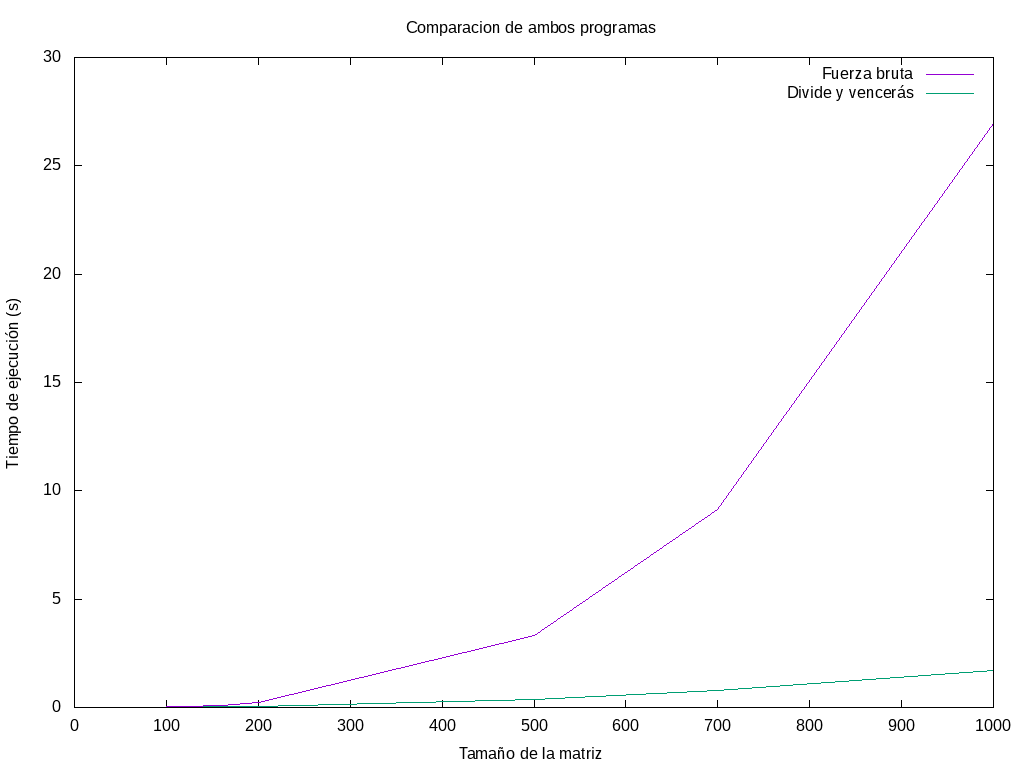
\includegraphics[width=0.7\linewidth]{../Codigo/Solucion/comparacion}
\caption{comparacion entre ambos }
\label{fig:comparacion}
\end{figure}


\end{frame}


\begin{frame}
	\frametitle{Comparación de nodos: ulysses5}
	
	\begin{table}[]
		\centering
	
		\label{my-label}
		\begin{tabular}{lllll}
	Técnica	& Branch and bound & Backtracking  &   \\
	N.totales& 120&120  &  &  \\
	N.podados&  35& 68 &  &  \\
	N.explorados&85  &52  &  &  \\

		\end{tabular}
	\end{table}
	
\end{frame}


\begin{frame}
	\frametitle{Comparación de nodos: ulysses8}
	
	\begin{table}[]
		\centering
		
		\label{my-label}
		\begin{tabular}{lllll}
			Técnica	& Branch and bound & Backtracking  &   \\
			N.totales& 40320&40320  &  &  \\
			N.podados&  38568& 37605 &  &  \\
			N.explorados&1752  &2715 &  &  \\
			
		\end{tabular}
	\end{table}
	
\end{frame}


\begin{frame}
	\frametitle{Comparación de nodos: ulysses10}
	
	\begin{table}[]
		\centering
		
		\label{my-label}
		\begin{tabular}{lllll}
			Técnica	& Branch and bound & Backtracking  &   \\
			N.totales& 3628800&3628800  &  &  \\
			N.podados&  3601453& 3566077 &  &  \\
			N.explorados&27347  &62723  &  &  \\
			
		\end{tabular}
	\end{table}
	
\end{frame}


\begin{frame}
	\frametitle{Comparación de nodos: ulysses12}
	
	\begin{table}[]
		\centering
		
		\label{my-label}
		\begin{tabular}{lllll}
			Técnica	& Branch and bound & Backtracking  &   \\
			N.totales& 479001600&479001600 &  &  \\
			N.podados&  478284703& 474474230&  &  \\
			N.explorados&716897  &4527370  &  &  \\
			
		\end{tabular}
	\end{table}
	
\end{frame}




\end{document} 
